\documentclass[10pt,twocolumn]{article}

% use the oxycomps style file
\usepackage{oxycomps}
\usepackage{csquotes}
\usepackage{graphicx}

% usage: \fixme[comments describing issue]{text to be fixed}
% define \fixme as not doing anything special
\newcommand{\fixme}[2][]{#2}
% overwrite it so it shows up as red
\renewcommand{\fixme}[2][]{\textcolor{red}{#2}}
% overwrite it again so related text shows as footnotes
%\renewcommand{\fixme}[2][]{\textcolor{red}{#2\footnote{#1}}}

% read references.bib for the bibtex data
\bibliography{references}

% include metadata in the generated pdf file
\pdfinfo{
    /Title (The Occidental Computer Science Comprehensive Project: Goals, Timeline, Format, and Advice)
    /Author (Dani Renteria)
}

% set the title and author information
\title{Game Genius: Improved Baseball Commentary}
\author{Dani Renteria}
\affiliation{Occidental College}
\email{drenteria@oxy.edu}

\begin{document}

\maketitle

\section{Introduction and Problem Context}

In this new dynamic landscape of contemporary sports, fueled by the emerging access to big data. The fusion of technology and athletics has unprecedented possibilities. Web applications nowadays are becoming increasingly more dynamic to keep up in this constantly evolving digital age. The question is how can we use this new access to data to develop web applications that can bring added excitement to modern sports? 

This project revolves around the world of baseball commentating. Baseball holds a special place in the hearts of millions all over the globe. Sports serves as a unifying force that transcends cultural and geographic boundaries. Recognizing this profound importance, my project aspires to elevate the sports commentating experience by providing not just mere statistics, but a new fast-paced narrative in the form of digitally created comments that attempts to dive deeper into the sport through the use of a web application.

The primary goal of this project is to provide a tool for MLB sports commentators to help reduce their preparation time and aid them while they're broadcasting live. The project aims to redefine the commentating experience by leveraging MLB game data to provide insightful and engaging commentary that pushes the boundaries of conventional sports coverage. Helping commentators in this way would not only aid some of the challenges they face while doing the job, such as long preparation time and quick on-the-spot thinking, but also provide a more engaging experience for aspiring commentators or even just baseball enthusiasts. The implications of this project are vast and future iterations have the potential to change the sports watching landscape for both commentators and avid baseball viewers. 
\break\break
The web application attempts to tackle these challenges:
\begin{itemize}
    \item \textbf{Difficult preparation for commentators}: Some of the initial preparation required will be replaced by a quick name look up in the web app. 
    \item \textbf{Improved organization}: The web application includes many features that allow commentators to generate, analyze, and organize their ideas and comments. 
    \item \textbf{New more engaging way to watch baseball}: Access to this app won't be limited to sports commentators. Fans can use the app in their own creative ways for added levels of enjoyment. 
\end{itemize}

\section{Technical Background}

In this section, all technical terms and topics necessary for the creation of this web app will be introduced and explained. \break\break
For starters, the development of the web application, built on the React framework, involves the use of JavaScript, HTML, and CSS to create an intuitive, organized, and dynamic user interface. React's component-based architecture facilitates modular designs, which enhance efficiency in development and aid code maintainability. The exact code architecture will be discussed in a later section. \break
\indent UX design was a big part of this project and is defined by Benoît Dabouis et al., in their article “Retrospective Coding of the UX Design Process for UX Design Enhancement in Design Agencies”, “as the perception of specific product attributes or qualities and the resulting effects on the user, such as emotions or behavior for example” (Dabouis et al. 2023). \cite{uxdesign} Part of the process required extensive design with the user's experience in mind and user testing - to be discussed in a later section- to make adaptations to those designs. Making web applications requires understanding the consumer well enough to serve their expected needs. Following this design framework was a primary goal since it directly mimics how design agencies create and enhance their products in the real world.
Moving on to the job of baseball commentators, it's essential to understand the process taken by a commentator as they prepare for games and matches. Beyond the quick play-by-play descriptions, commentators dive into extensive research, inspecting player statistics, team dynamics, and even historical context. Professional commentators also often have a team behind them helping facilitate their preparation. This complex overview ensures that the commentary not only narrates the game but also provides an insightful analysis that improves the viewer's understanding and appreciation of the sport. Like stated earlier, a goal of the web app is to help ensure this preparation process runs smoothly. \break
\indent Finally, understanding basic baseball statistics is beneficial for comprehending some of the comment structure. Metrics such as batting averages, and on-base percentages for batters, and earned run averages (ERAs) for pitchers serve as the quantitative foundation for insightful commentary. These are basic metrics calculated by using data from historical game performance (including but not limited to at-bats, hits made, innings pitched, etc). The web application aims to seamlessly integrate these statistics for the commentator, providing users with a comprehensive and data-driven perspective on the game as it progresses. 



\section{Prior Work}

Analyzing past and similar works is crucial as part of a product improvement process. This section provides a background on related topics and literature that contributed to part of the application design. \break\break
\indent A sports commentary web application can draw parallels with traditional sports journalism, where some of the insightful preparation and work done are very similar to a commentator. Even more interesting, however, is the use of AI and Natural Language (NL) Models such as ChatGPT to generate manuscripts in sports and exercise medicine (SEM). In an article titled “AI did not write this manuscript, or did it? Can we trick the AI text detector into generated texts? The potential future of ChatGPT and AI in Sports and Exercise Medicine manuscript generation” from the journal \textit{BMJ Open Sport and Exercise Medicine}, author Nash Anderson discusses some of the implications, both negative and positive, AI can have on the future of text generation. 

\begin{displayquote}
Natural language model-based AIs, such as ChatGPT, are tools to watch for generating natural conversational text for various manuscript contents in SEM. However, ethical, equity, accuracy and detection concerns associated with their use are potential threats to scientific integrity. (Anderson 2023)
\end{displayquote}
\cite{nash2023}

Part of the authors discussion in the study revolved around the potential issues that might arise from using AI to write. AI journalism has been prone to plagiarism in the past. When using NL models, yes some of the generated texts can be useful and well written, but it comes with a multitude of issues, some even being overall accuracy. When designing this project, AI was a potential piece of the puzzle to use to generate insightful commentary. They would use the stats to create “creative” comments of their own. However, in the end, I decided for the first iteration of the application that it might be simpler to design and structure the comments by hand. Using AI in the future will require developers to carefully understand ethical issues and increase their development cycle as they’ll have to devote more time to ensure the NL models are properly integrated to mitigate risk and reduce inaccuracies. \break
\indent AI is still seeing improvements and adaptations. Which is why most of the preparation work for commentators is still done with more traditional tools. Stat encyclopedias have long served as repositories for numerical player data. The type of information in these encyclopedias created the foundation of the comments seen in the application. Since AI wasn't used, the web application uses historical stats to present to the commentator quickly while also re-calculating live during a game. Stat websites like baseball-reference, fangraphs, and even MLB themselves influenced not only the designs of the app but the purpose as well. I wanted the application to go beyond traditional numerical stats and attempt to provide new perspectives. \break
\indent This attempt to move past tradition was a big part of the project. By looking into AI and changing the way stats are presented, the project was moving in a new direction that hoped to change the job of sports commentating. Another place for inspiration came from modern social media usage for sports journalism. In an article titled, “There He Goes: The Influencer–Sports Journalism of Fabrizio Romano on Twitter and Its Implications for Professionalism”, author Simon McEnnis discusses how sports influencers use social media professionally and responsibly to present their ideas and objective news. 

\begin{displayquote}
This article explores Romano’s Twitter practice to provide a vital insight into how an influencer–sports journalist approaches professionalism. The sociology of professions has emerged as an important conceptual framework in understanding journalism change in the digital age. (McEnnis 2023)
\end{displayquote}
\cite{mcennis2023}

McEnnis' analysis provided two main ideas. One being the modern use of Twitter for sports journalism, and the second being this sociological framework. Romano’s story brought to light the truth behind the future of sports analysis and broadcasting. In recent years, we’ve seen the role of social media change drastically. Once seen as a simple form of entertainment, it is now a complex and powerful tool to connect millions of people. Although social media wasn't directly a part of this project, it was an inspiration. This shift towards more modern approaches to sports watching is what started this project in the first place.

\section{Methods}

This section of the paper will dive into the methodology employed for building the web application, highlighting the personal touch brought to the process through interviews, UI design, data preparation, effective implementation with React, and the critical phase of testing. Each subsection will showcase the specific strategies and considerations that were key phases of development.

\subsection{Interviews}

Prior to design and implementation, in order to fully understand the needs of the users, interviews were conducted with collegiate sports announcers/ commentators in an attempt to get a glimpse into the sort of preparation they do for games. \break\break
The main sections for this process were as follows:

\begin{itemize}
    \item \textbf{Step-by-step preparation process}: What do they do to prepare and how long is the process?
    \item \textbf{Information relevant to the job}: Besides sport statistics what other information do they try to bring up? 
    \item \textbf{What it takes to be a sports announcer/ commentator}: How is their presence “in the stands” different from normal? Can anyone be a sports announcer?
\end{itemize}

Conducting this type of interview allows me to better equip the application with features that would aid the user. It also helped go beyond normal statistics and push different types of comments. Throughout this process, it was understood that broadcasters don't just recite performance metrics. They attempt to connect with the player in order to provide a more personal and entertaining experience for the audience. The job of a commentator is also similar to TV hosts in other fields. Being “on tv” means establishing a quality presence that is professional yet fun and entertaining. This is, of course, hard to translate into the app but the overarching goal here was to ensure the application will not impede this process for the commentator. Instead the level of organization displayed in the app will allow the commentator to focus more on their presentation. \break
\indent This interview process helped me set requirements for the final version of this project. 

\subsection{UI Design}

Once interviews were completed and discussed, the next phase of this project was initial user interface designs. The main goal here was to create a user-friendly interface that will improve a commentator’s job while maintaining a professional appearance and overall organization. Nowadays, designing interfaces can be a challenging task. The reason for this is in the dynamic nature of modern web applications. In a book titled \textit{On the Separation of User Interface Concerns : A Programmer's Perspective on the Modularisation of User Interface Code}, author Sofie Goderis discusses some of the difficulties and concerns when it comes to developing a well functioning user interface. Much of her initial discussion was on the overall flexibility of modern interfaces. “While a high-degree of variability will allow software to be reused in a broader range of contexts, it implies that the implementation needs to exhibit a high degree of flexibility” (Goderis 2008). \cite{sofie2008} This high degree of flexibility is what makes designing a hard task. Web applications have been transitioning, over the last few years, to more sleek, innovative, and creative designs to appeal to new generations while maintaining a seamless experience for all users. \break
\indent For these reasons, there were a number of changes made throughout the design process. For example, I switch from a multi-page design with individual pages for batters, pitchers, and teams, to a side by side panel design that would allow commentators to quickly input “events” - to be discussed in the implementation section- and see resulting comments on the side (shown in figure 1 and 2) improving efficiency. 
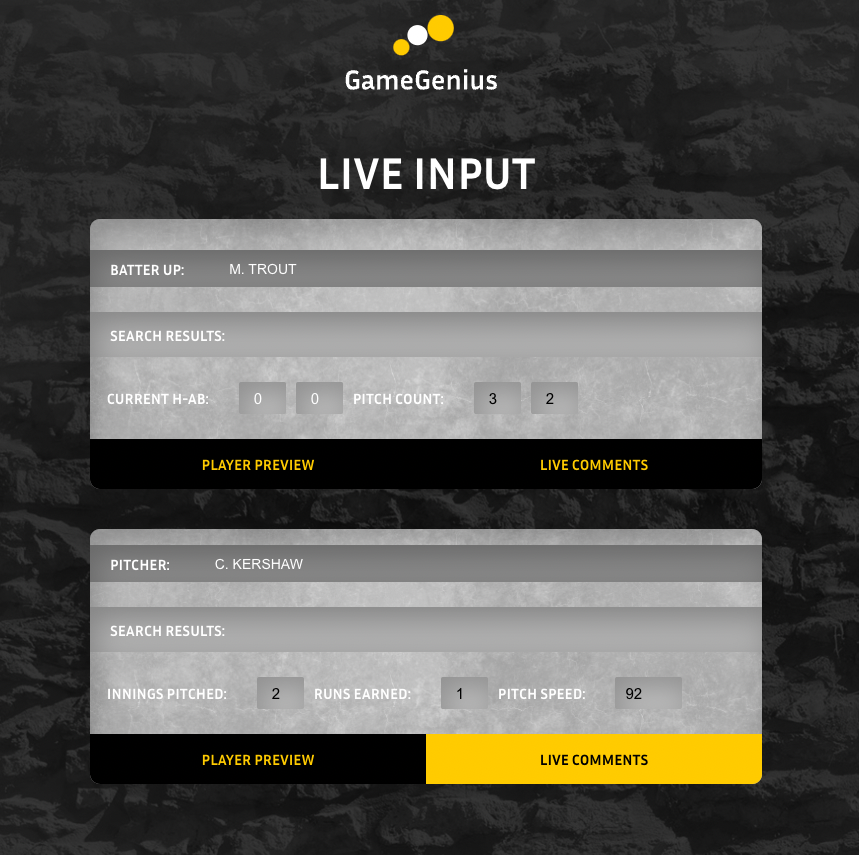
\includegraphics[scale=0.24]{images/input.png}

\textit{Figure 1: Input field. }

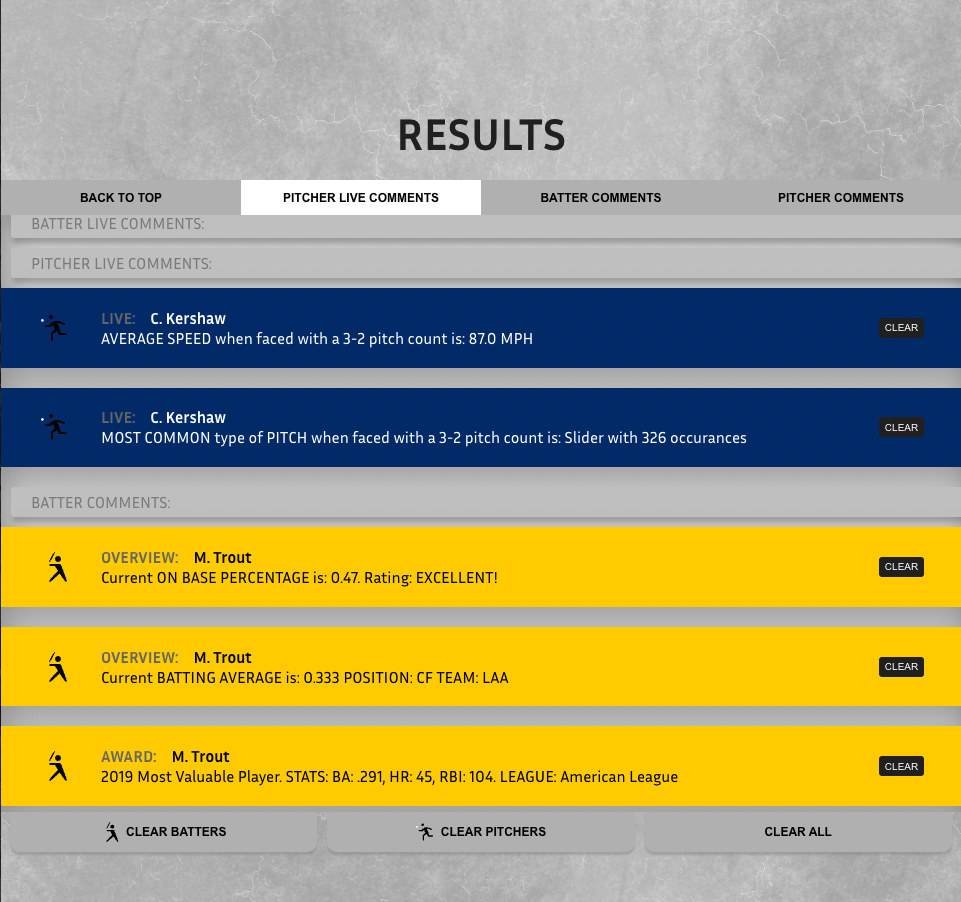
\includegraphics[scale=0.20]{images/results.png}

\textit{Figure 2: Results field.}

The prototyping for this project took place in Figma, a cloud-based design and prototyping tool. Using Figma allowed me to easily make modifications to components or add new ones entirely before coding is even required. 
Additionally, after the design process was completed, some features were changed and adapted to fit new unexpected needs. These adaptations were based on early user testing with the Figma mock-ups (shown in figure 3) - more specific user testing will be discussed in a later section of this paper.

Overall, this part of the development cycle is crucial to the success of the application. Much time was spent on this step to minimize the potential changes that would have slowed down development. 

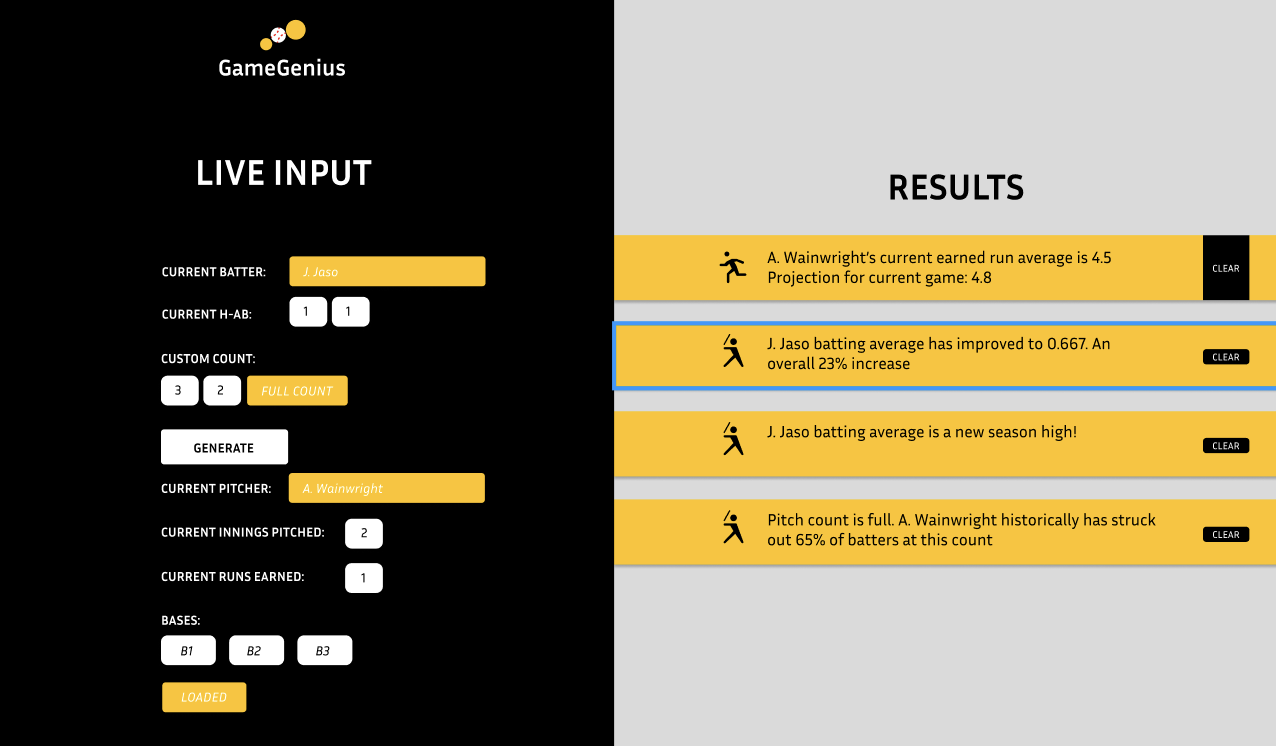
\includegraphics[scale=0.3]{images/initial-designs.png}

\textit{Figure 3: Initial Designs}

\subsection{Data and Preprocessing}

Gathering and preparing data came with many challenges - along with ethical concerns to be discussed in a later section. This part of the process was broken down into two main sections:

\begin{itemize}
    \item \textbf{Sourcing data and discussing reliability}: Once data was found, there needed to be a thorough analysis on the data to make sure information was accurate
    \item \textbf{Data clean up}: Once the source was approved, data had to be processed prior to usage
\end{itemize}

The data was sourced from an open data set found on Kaggle. The data set contained information on how the data was gathered and from where. The data set we used was titled “MLB Game Data” and was scraped directly from ESPN’s own records and had a usability score of 8.24. Note this usability score describes how easy the data is to work with and overall usefulness (helpful and accurate). There were discussions over this score and what it meant for the app. But for the purposes of this project, it was decided that that state of the data set - although not perfect - would fit the requirements for the web application. \break
\indent Once the data was found and looked over, it was time to figure out what files were needed for comments and what files needed to be adapted. The CSV files chosen for this project from the data set were as follows:

\begin{itemize}
    \item \textbf{hittersByGame}: Information on batters and their respective statistics
    \item \textbf{pitchersByGame}: Information on pitchers and their respective stats
    \item \textbf{pitches}: Data on every single pitch thrown since 2016-2021
    \item \textbf{MVP}: Historical MVP awards
\end{itemize}

The pitches and MVP files were the two that needed to be changed or modified for quicker and easier lookup in preparation for the implementation process. The pitches file had challenges due to the size. Therefore some of the unnecessary attributes present in the file (like play-hitzone,  play-field, etc) needed to be removed to reduce file size -attributes were removed with the use of a Microsoft power query. Although this step isn't ideal, it was necessary for the initial success of the project. Future use of a database will be discussed in a later section. \break
\indent The MVP file was reformatted to a single dataset - original format had leagues separated (American and National League). Once these files were checked and processed, the implementation step could proceed. 

\subsection{React Implementation}

Having a detailed design and data prepared made the start to the implementation process easier to handle. I chose to use React for two specific reasons. One being my overall comfort level with the library since I've used it before in past projects. I wanted to make sure I had a good grasp at the basics. The second reason I chose React was because of its large and active supportive community and its easy to understand JSX (a React syntax extension that's similar to HTML). Having this community made it easy to look for help when confronted with barriers and challenges through the process. And JSX syntax makes it easier to write and understand HTML code which is crucial for web development. React has a component-based architecture which allows developers to separate parts of the application for organization and debugging (see more in the code architecture section). Although this project isn't as modular as I expected, it does leave room for improvements in future iterations.

The implementation process was made simpler since Figma was used to create the designs. Meaning much of the CSS styling could be extracted from the mock-ups in Figma’s developer mode. Of course there were style changes made throughout the process but Figma was consistently used to aid in implementing those changes. The actual structure of the app is separated into two different components: the app itself and the input and output container. Projects are usually separated like this to style components globally or locally. 

The process was broken down as follows: 

\begin{itemize}
    \item Input fields: creating simple yet effective input forms for commentators
    \item File parsing and reading: on submission, necessary files would be fetched and parsed for data extraction or recalculation
    \item Structuring comments: data was formatted into a comment to be displayed as a result
\end{itemize}

The exact structure and code to be discussed and visualized in a later section.

Overall, this implementation process was a big part of the project that required extensive preparation and execution. In order for the comments to work, I needed to make sure that the data from the files was being read properly and its attributes were used correctly to ensure a level of accuracy appropriate for the application. That meant testing sample data extraction calls and calculations to make sure my method calls were done correctly.  

\subsection{User Testing}

After initial implementation of the project was done, it was time for user testing. This step is crucial to know the project is serving the expected audience. There were many challenges trying to acquire commentators to look at the application however. Therefore, after much consideration, users for the test were chosen based on their current MLB knowledge instead. The testing was conducted to gain feedback on not only the interface, but the comments themselves. 

The initial feedback given can be organized into two main topics: 
\newline
\textbf{Design Aesthetics and Usability}: 

\begin{itemize}
    \item Input fields were simple enough to understand and use quickly
    \item Since there were separate fields for batter and pitchers some of the users believed certain inputs like pitch count worked better as a pitcher input rather than a batter
    \item Liked the professional looked obtained and level of organization
\end{itemize}

\newline 
\textbf{Comments}: 

\begin{itemize}
    \item Player preview comments were basic but required. Some users wished there were more personal and historical comments, however, this was difficult to address due to the limitations posed by the chosen data source
    \item Scrolling was made easier with the aid of locator buttons but without instruction some of the added convenience was lost 
\end{itemize}

This feedback for comments was expected but, as stated before, due to the nature of the data, there were some types of comments that were unavailable to structure at the time.

\subsection{Conclusion}

To conclude this section, the implementation of the outlined methods produced a successful and user-friendly web application that seamlessly integrates insightful baseball commentary with user-driven commentator input. The interviews, complex UI design, and user testing have collectively contributed to a positive user experience. However, it is crucial to recognize that the project doesn't end here. Future iterations hope to incorporate even more comprehensive data to refine statistical analyses and comments for added depth and a new level of entertainment. 

The hope of this project is to open the door to new sports as we get better at gathering necessary data. 

\section{Evaluation Metrics}

In this section, the metrics and methods used to evaluate the web application will be described and discussed in terms of their objectives. This process is best defined by author Luis Olsina et al. in chapter 13 of their book titled “How to Measure and Evaluate Web Applications in a Consistent Way”.

\begin{displayquote}
    A measurement or evaluation process prescribes or informs a set of main phases, activities, and their input and output that might be considered. Usually, it says what to do but not how to do it; that is, it says nothing about the particular methods and tools in order to perform the specific activities’ descriptions. 
(Olsina et al. 2008)
\end{displayquote}
\cite{olsina2008}
For this project, the metrics chosen attempted to measure usability and functionality, and content and reliability.

\subsection{Usability and Functionality} 

This section aimed to evaluate the ability for the user to understand the application and all its features. It also functioned as a measure of the ability to quickly learn how to use the interface without extensive instruction (\textit{shown below in figure 4}).

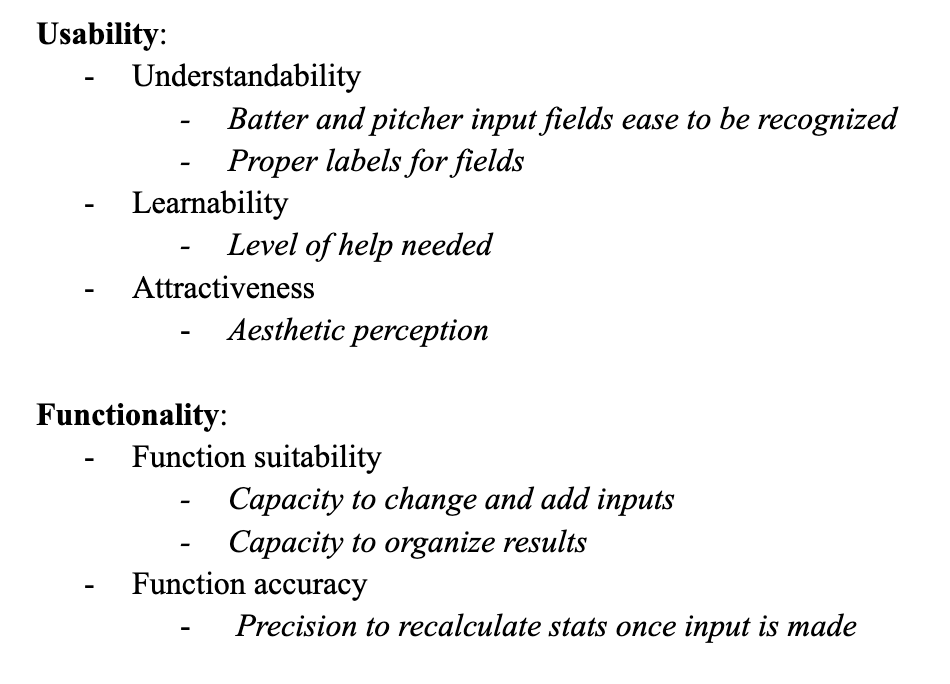
\includegraphics[scale=0.50]{images/usability.png}

\textit{Figure 4: Usability and Functionality Metrics.}

\subsection{Content and Reliability}

This section aimed to evaluate the content produced by the application and reliability in regards to its overall accuracy (\textit{shown below in figure 5}).

Both these metrics were scored by users while navigating through the app and all of its features. Besides an overall introduction on the app, no other instruction was given. 

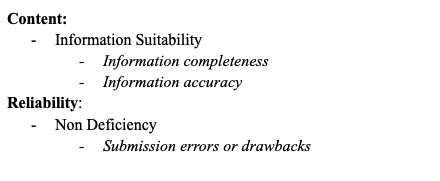
\includegraphics[scale=0.50]{images/Screen Shot 2023-12-14 at 7.57.28 PM.png}

\textit{Figure 5: Content and Reliability Metrics.}
\break

\textit{These metrics were chosen based on traditional web application testing and evaluating processes highlighted in the Olsina reading above. }

\section{Results and Discussion}

This section will walk through the results from the metrics used to evaluate the project as well as some of the possible solutions that can address issues in future work. 

\subsection{Usability and Functionality Results}

All users respond positively to the input fields following the metrics shown in figure 2.1. For an avid MLB fan, the labels shown in the input fields were easy to understand and values were easy to update.

Efficiency was a goal of the project and all users appreciated the side-by-side design that allowed them to look at results and input values at the same time. The only drawback was in the overall organization of the methods employed after submission that resulted in slower generation times. Each method fetched one or two csv files and ran a search through each row to gather information on a specific player by matching input name. This process was slow for some larger files like \textit{pitches.csv} for reasons discussed earlier. Future iterations of this project might benefit from a custom database that will allow faster look up and more holistic comments due the increased available data.

From an aesthetic perspective all users respond positively to the layout and color scheme.

\subsection{Content and Reliability Results}

Most users responded positively to the overall structure of the comments in terms of their overall relevance to the sport. Users seemed excited by the comment generation. During this evaluating process there were no signs of submission or fetching errors. 

Accuracy here was a main talking point. Since the data was sourced by a third party and it was almost impossible to verify its entirety, some of the stat values drew minor concern. Although numerical accuracy was/is of vital importance, there were some compromises that were made to ensure a working final product. Future iterations will require more extensive data verification that would compare different data sources to find and resolve any discrepancies. Given a longer time frame, this part of the process would be revisited.

Overall this evaluating process ran smoothly and resulted in specific and feasible changes that will improve the overall success of the application. 


\section{Ethical Considerations}

This section will explore the ethical considerations made throughout the development process of this web application. This section will primarily focus on responsible data collection, the importance of accuracy in statistics, and adherence to professional journalism standards. 

With any project that uses big data, there are a multitude of ethical issues that need to be addressed. But what exactly constitutes a big data project? Defined by author Wenhong Chen, in his article “Big Data Ethics and Politics: Toward New Understandings”, “big data encompasses any and all structured and unstructured information collected, stored, linked, and analyzed either online or offline” (2020). \cite{chen2020} For this project, I'm referring to the MLB game data that serves as the foundation for the web application. The main ethical concern that came up was regarding the way in which the data was sourced and collected. According to Chen, there are two main aspects to look out for when working with big data: “potential biases in big data collection and interpretation, [and] community and citizen concerns of big data (mis)use in public life and for journalistic purposes” (2020). 

As I stated before, the data used was found in an open data set on \textit{Kaggle}, which is an online platform that provides free access to data sets for research purposes. Sourcing data ethically can be a tricky task, especially if the data comes from big corporations such as ESPN. Although there probably won't be any bias present sourcing from a company with a reputation like ESPN’s, there are calls for concerns in the way the data might be used. When collecting it's important to abide by the usage terms which companies set for their information. There are all sorts of legal issues that may arise if data is scraped and used incorrectly. Typically using public data sets like this one is fine as long as the project doesn't revolve around selling a product - no monetization no problem.  However there are other issues that come with using public data sets. 

Information accuracy is also a big call for concern when using open data sets from \textit{Kaggle}. Since the data was scraped by a third party- the owner of the data set- it's hard to verify the level of accuracy achieved by their work. Accuracy is the primary metric of success in statistics. There is no numerical misinterpretation when a batter hits a run or a pitcher strikes someone out. It's simply an uncontested numerical record. Having wrong or inconsistent records is an issue since the web application uses those records to form quality comments. Using false data will cause misrepresentations of player performances ruining the reputation of the app. For this project, it's important to discuss the limitations and assumptions made of the data to users prior to usage. That way we maintain transparency in the way we tackle accuracy concerns.

Finally, since this project revolves around sports commentating, it's important to look into professional journalism standards as the two jobs share similar objectives. More importantly, what are some of the contemporary issues sports journalists face as part of their job, and how are these relevant to a sport commentary web application? 

The main issue I would like to discuss is navigating personal bias when representing players online or on air. In an article by authors Jessica Kunert and Kuni Peer titled “Tension between Journalistic and Entertainment Values in Live Soccer TV Commentary: The Commentator’s Perspective”, they discuss the challenge commentators and journalists face when evaluating their own job performance. “While the sports journalists’ main desire has been found to inform their audience in a neutral and precise way, like their counterparts from other beats, providing entertainment and relaxation to the audience is also a high priority” (Kenert and Peer 2023) \cite{kunert2023}. Here the authors point out an important distinction between job objectives. On the one hand, commentators and journalists should aspire to represent players equally and respectfully regarding their performance. That means removing all bias and opinions. But on the other hand, commentators should aim to be energetic and entertaining when “preforming”. From an ethical perspective, when in a position of influence, it's crucial that a person (commentator) stay aware of their personal stances in order to reduce the negative effects of biased journalism. Including but not limited to alienation of fans, damage to player reputation, and diminished credibility. 

Since the web app creates comments for a commentator, part of the comment design process involved removing bias and focusing on stating facts. The application wasn’t designed to replace a commentator but instead allow them to focus on providing the excitement to the game. A main goal of the project was to avoid perpetuating unwanted bias. 

By addressing these ethical issues and concerns prior to the final product presentation, the web application not only aligns with industry best practices but also ensures the trust and satisfaction of all of its users. Addressing challenges and barriers both ethical and technical is a crucial step in the process of building modern web applications. 

\section{Code Replication}

Project was built using react version 18.2. (\textit{only additional package used was pandas to parse and read CSV files})

\section{Code Architecture}

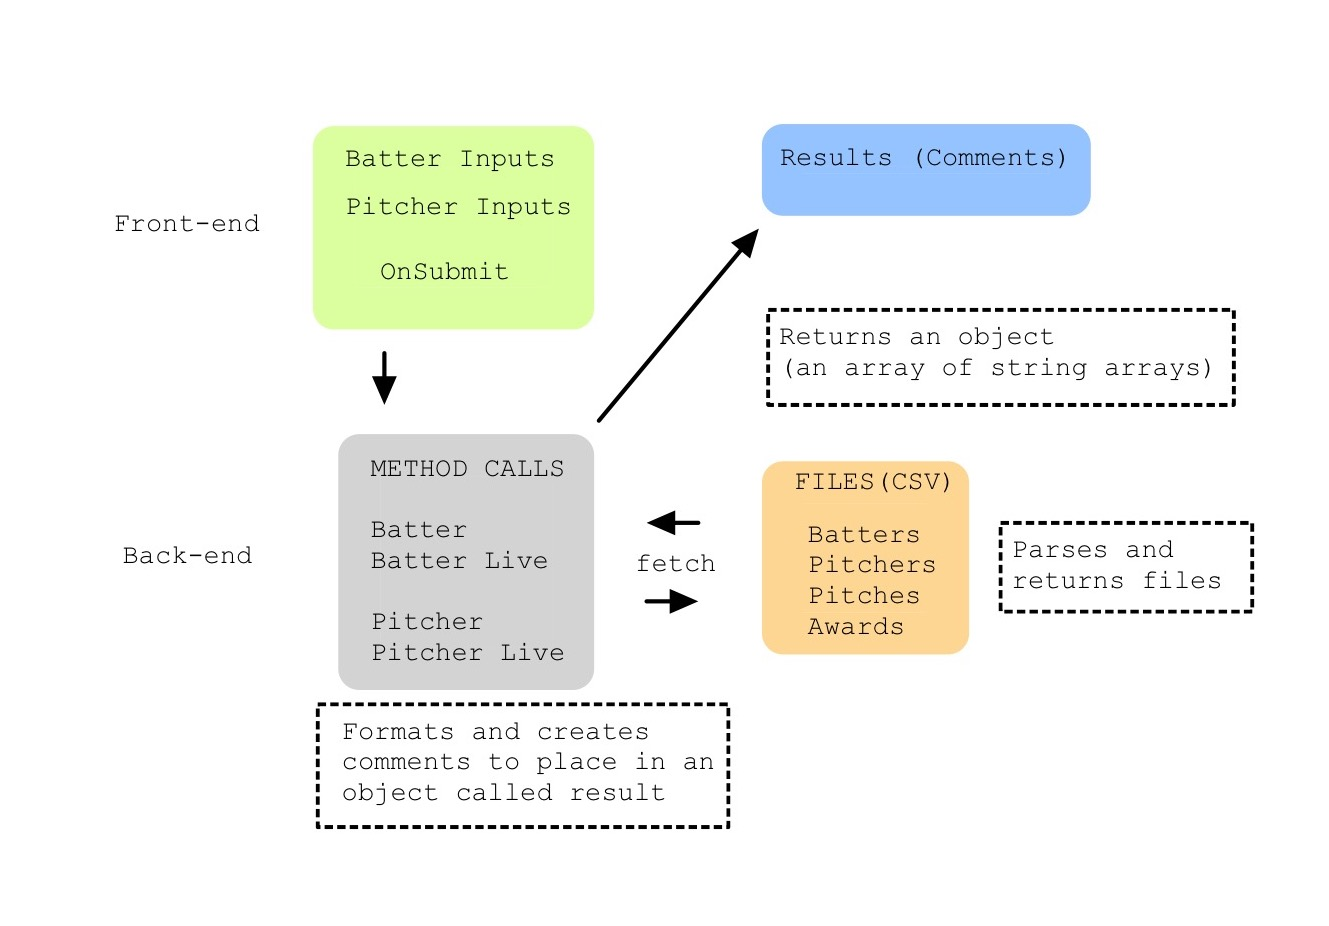
\includegraphics[scale=0.20]{images/arch.jpg}

\textit{Figure 5: Code Architecture}
\newline
Here is a visual representation on the structure of the application. Showing input fields in the front-end and results in the back-end along with method calls inbetween. 

\printbibliography

\end{document}
